\documentclass[conference]{IEEEtran}
\IEEEoverridecommandlockouts
% The preceding line is only needed to identify funding in the first footnote. If that is unneeded, please comment it out.
\usepackage{cite}
\usepackage{amsmath,amssymb,amsfonts}
\usepackage{algorithmic}
\usepackage{graphicx}
\usepackage{textcomp}
\usepackage{xcolor}
\def\BibTeX{{\rm B\kern-.05em{\sc i\kern-.025em b}\kern-.08em
    T\kern-.1667em\lower.7ex\hbox{E}\kern-.125emX}}
\begin{document}

\title{Real-Time Monitoring and Remote Guidance of\\ Mobile Robots Using Multimodal Digital Twins}

\author{\IEEEauthorblockN{Trung Kien La}
\IEEEauthorblockA{\textit{Dept. of Comp. Science \& Engineering} \\
\textit{Frankfurt University of Applied Sciences}\\
Frankfurt a.M., Germany \\
trung.la@stud.fra-uas.de}
\and
\IEEEauthorblockN{René Harmann}
\IEEEauthorblockA{\textit{Dept. of Comp. Science \& Engineering} \\
\textit{Frankfurt University of Applied Sciences}\\
Frankfurt a.M., Germany\\
rene.harmann@fb2.fra-uas.de}
\and
\IEEEauthorblockN{Eric Guiffo Kaigom}
\IEEEauthorblockA{\textit{Dept. of Comp. Science \& Engineering} \\
\textit{Frankfurt University of Applied Sciences}\\
Frankfurt a.M., Germany \\
kaigom@fb2.fra-uas.de}

}

\maketitle

\begin{abstract}
    Although digital twins have been playing a pivotal
    role in the management of the lifecycle of physical robotic
    systems of systems, they have hardly been employed to guide
    mobile robots in real-time. In fact, the guidance of such systems
    requires functionalities, including the perception of targeted
    locations and avoidance of collisions, that build upon spatial
    information beyond internal robot states usually acquired using
    proprioceptive sensors. In this case, exteroceptive sensors help
    meet this demand. Nevertheless, such sensors have received little
    attention thus far in the development of digital twins. On the
    other hand, the completion of various spatial objectives, such as
    reverse motions, might require the awareness of the historical
    internal state of the distant robot. For instance, the current
    energy budget is likely to constrain the reachability of the
    initial state after a while, even when spatially and kinematically
    feasible. We therefore embrace these challenges with a multi-modal 
    approach to provide and employ digital twin of mobile robots. 
    We collect data about the internal state and camera-
    captured neighborhood of the robot in real-time. The robot
    operator is thereby provided with a multi-dimensional state and
    perception view that characterizes the robot, elevates situational
    awareness, and facilitates decision support. We then develop a
    versatile graphical interface that helps monitor and steer mobile
    robots. Since the bidirectional approach is intuitive and user
    friendly, even novices can remotely guide a mobile robot with
    multi-modal situational awareness. We show the versatility and
    effectiveness of our approach in use case scenarios in practice.
\end{abstract}

\begin{IEEEkeywords}
    Robotics, Multimodal Data, Digital Twins, In-
    dustry 4.0, Industry 5.0, Society 5.0, Human-Mobile Robot-
    Interaction, Systems of Systems
\end{IEEEkeywords}

\section{Introduction}
The Robot Operating System (ROS) stands as a ubiquitous middleware framework in the realm of robotics serving as a foundational platform for constructing robot systems and developing robot applications \cite{rosOrg}. 
However, for individuals possessing limited or no prior exposure to robot software, navigating the intricacies of ROS can prove challenging. 
This challenge is particularly pronounced for users who rely on robotic assistance and require an intuitive means of interacting with these machines.
In response to this need, we have developed a platform-independent web application. 
Designed with accessibility in mind, this application facilitates seamless monitoring and control of a locally networked robot. Users gain access to critical information, including battery status and motor temperatures, all presented through an intuitive web interface. 
\begin{figure}[htp]
    \centerline{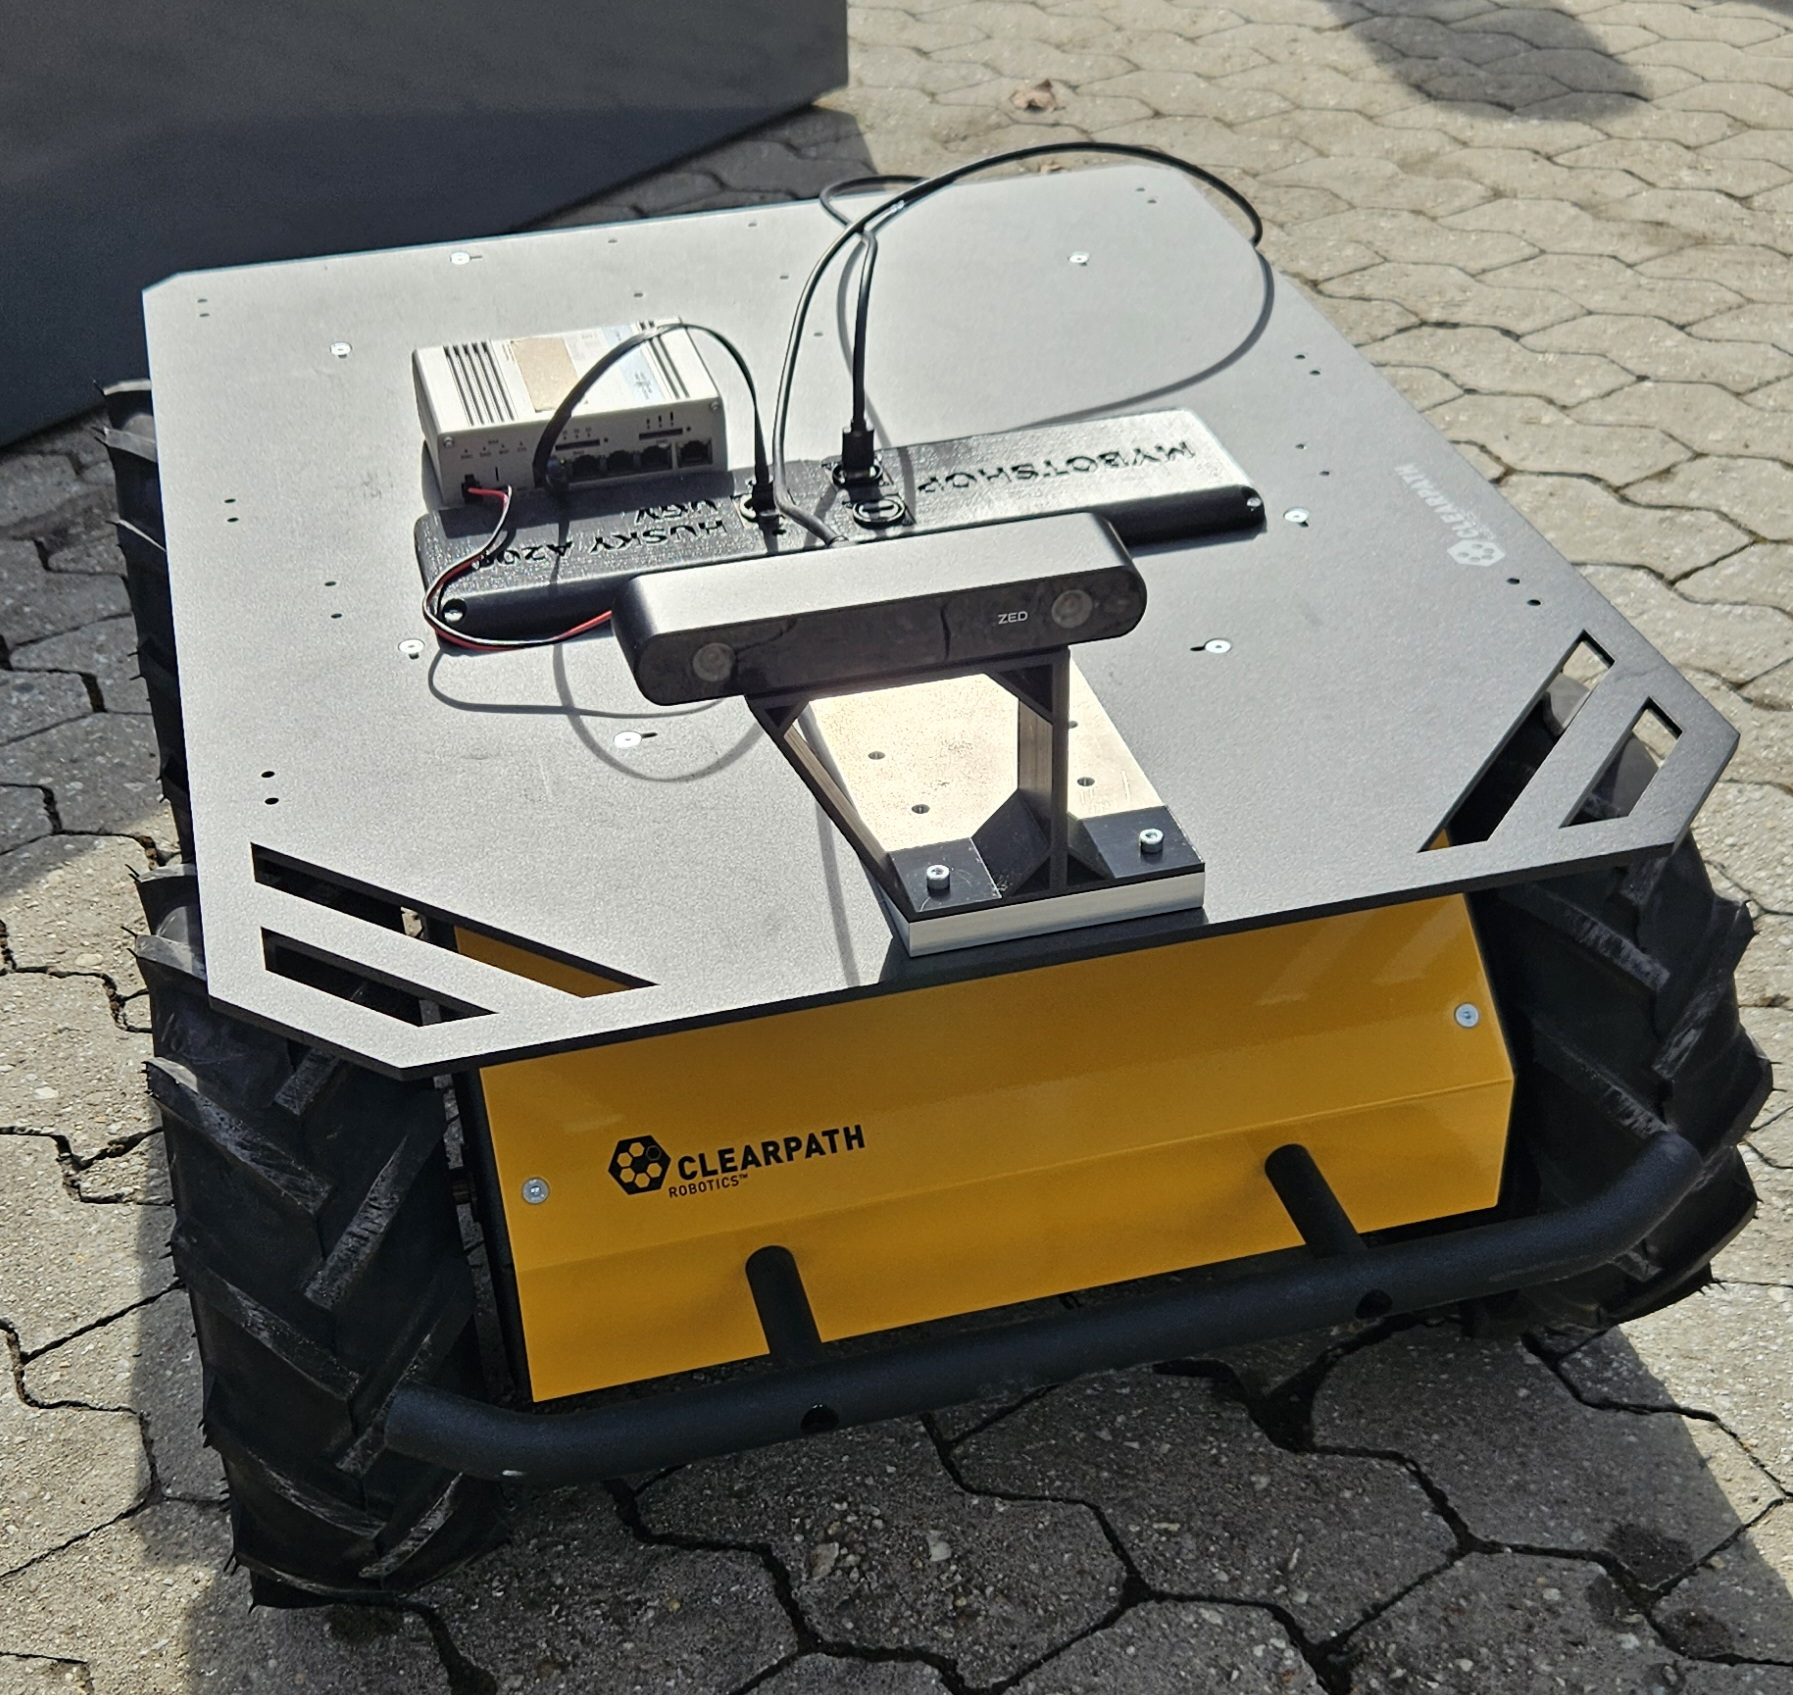
\includegraphics[width=8.9cm]{Pictures/huskyzed2.jpg}}
    \caption{The Husky UGV by Clearpath Robotics with an attached Zed 2i stereo camera}
    \label{fig:huskyClearpath}
\end{figure}
Notably, this application is compatible with any device supporting web browsers, ensuring widespread accessibility and usability.
The robotic platform employed in our research is the Husky Unmanned Ground Vehicle (UGV) manufactured by Clearpath Robotics. This medium-sized mobile robot depicted in Fig. \ref{fig:huskyClearpath} operates on the ROS2 distribution Humble Hawksbill.
The Husky UGV boasts a substantial maximum payload capacity of 75 kg rendering it suitable for transporting and accommodating various auxiliary components. Researchers can mount additional robots, peripherals and specialized tools on this versatile platform. Its robust design and adaptability make it an ideal choice for a wide range of robotic applications\cite{huskyClearpath}. 

\section{State of the Art}
In \cite{kapic} a Python web application was developed with the Django framework that uses a single virtual joystick with the objective to teleoperate the TurtleSim robot within a simulation environment. 
A WebSocket connection and the ROS JavaScript library Roslibjs were used to send commands from the web application to the robot. Specifically, the web application dispatched a twist message comprising of vector components representing both linear and angular motion to the robot. This message effectively guided the robot's movements, enabling teleoperation.
The Rosbridge protocol constitutes a pivotal component within the ROS ecosystem. In form of a ROS package (rosbridge\_suite) it includes a WebSocket server and uses the Roslibjs library. Its primary purpose lies in establishing a robust foundation for communication, leveraging the JavaScript Object Notation (JSON).
In practical terms, the Rosbridge protocol enables programming languages proficient in handling JSON to engage in effective dialogue with ROS via the Rosbridge. 
This enables external systems and applications to perform certain operations, such as subscribing to or publishing ROS topics \cite{rosbridgeOkState} \cite{rosbridgeSuite}.\\
In \cite{dinodi} a web application was developed with the primary objective of moving a Turtlebot3 in a virtual simulation environment with image transmission and autonomous navigation options. A virtual joystick was also made available to the user for manual control. Similarly to the first application, the communication between the app and the Turtlebot3 is facilitated with Rosbridge. 
One of the core aspects of the app is to bring robots closer to beginners and those interested in ROS. 
The app makes use of a range of frameworks and ROS-specific software. Among others, ReactJS, a JavaScript library was used for the frontend and to create the virtual joystick. For the backend, NodeJS and ExpressJS frameworks were used to open the ROS simulation environments. 
The authors state that only minimal knowledge of robotics is required to use the application. The app is also accessible to anyone with web access.\\
In \cite{johnson} a web platform was developed that deals with social robot application development. A physical Baxter robot and a virtual Baxter robot in the Gazebo ROS simulation environment were used. In essence, it is about web-based interpretation of social signals, hybrid block/text scripting interfaces and ROS integration via Rosbridge. 
The web components were created using JavaScript. The Baxter robot is equipped with a camera whose video stream is accessible to users via the ROS package web\_video\_server \cite{webvideoserver}.\\
A live remote interaction platform called TeleRobot was developed in \cite{wang}. This is also based on Rosbridge to interact with serveral robots and WebRTC to transmit images and audio in real-time. The main focus of this platform is to make robots accessible to users. The robots are controlled via a control panel. Other features include live chat, live streams, user management and an integrated database.

\section{Implementation and Design}
The system architecture of our web application can be dichotomized into distinct backend and frontend components. These components synergistically leverage an array of tools and frameworks to facilitate seamless operation.
Fig. \ref{fig:loop} illustrates the general idea of the data loop between the Husky UGV robot and the web application.

\subsection{Backend}
Our web application is built using Flask, a micro web framework designed for Python.
Flask offers core features and extensions to swiftly develop web applications. Flask is also very flexible and highly expandable \cite{flasksqlite}. The following tools are used in the backend:

\begin{itemize}
\item SQLAlchemy is a Python SQL toolkit and can be integrated into Flask as an extension. SQLAlchemy allows users to link Python objects to SQL databases using Object-Relational Mapping (ORM). This allows, for example, database queries to be made using Python code instead of SQL commands. The extension is also database-agnostic. 
Python code can be used unchanged for various SQL-based databases such as SQLite, PostgreSQL or MySQL \cite{sqlalchemy}. 
SQLite is used as a database to store ROS and user data. SQLite is a serverless database. It directly performs read and write operations on standard disk files. This characteristic renders it operable in a self-contained manner, devoid of any supplementary software dependencies or intricate configuration settings. Consequently, it exhibits resource efficiency by minimizing the utilization of extraneous computational resources \cite{sqlite}.
\item The Roslibjs JavaScript library and the Rosbridge v2.0 protocol are used to establish bidirectional communication with the robots and the web application. The Rosbridge server it contains, provides a WebSocket connection so that web browsers can communicate with Rosbridge.
Roslibjs is employed as a JavaScript library to interact with ROS topics, enabling the subscription to and publication of these topics \cite{rosbridgeOkState} \cite{rosbridgeSuite}.\\ A quintessential example of this interaction is the publication of a geometry\_msgs/Twist message on the /cmd\_vel topic of the Husky robot which initiates its movement.
The geometry\_msgs/Twist message is composed of linear and angular vectors, which represent the velocity in free space \cite{twistmsg}. Specifically, these vectors are expressed in terms of meter per second and radian per second, respectively, in a right-handed coordinate system.
In the context of the Husky robot, a linear velocity of 1 meter per second in the positive x-direction corresponds to forward movement at a speed of 1 meter per second. To induce rotational movement, an angular velocity is specified in the z-direction \cite{huskydriving}. Positive and negative values correspond to counterclockwise and clockwise rotations respectively.
\item The Web Video Server is a ROS package that allows HTTP streaming of ROS image topics \cite{webvideoserver}. This integrates the live image from a Zed 2i camera from StereoLabs into the web interface.
\item Flask-Login and Werkzeug.security extensions are used to handle login, logout, and session functions as well as to enhance user password security through password hashing \cite{flasklogin} \cite{werkzeug}. Additionally, it is possible to register new user accounts and assign permissions to different user roles. 
\end{itemize}
\begin{figure*}[htbp]
    \centerline{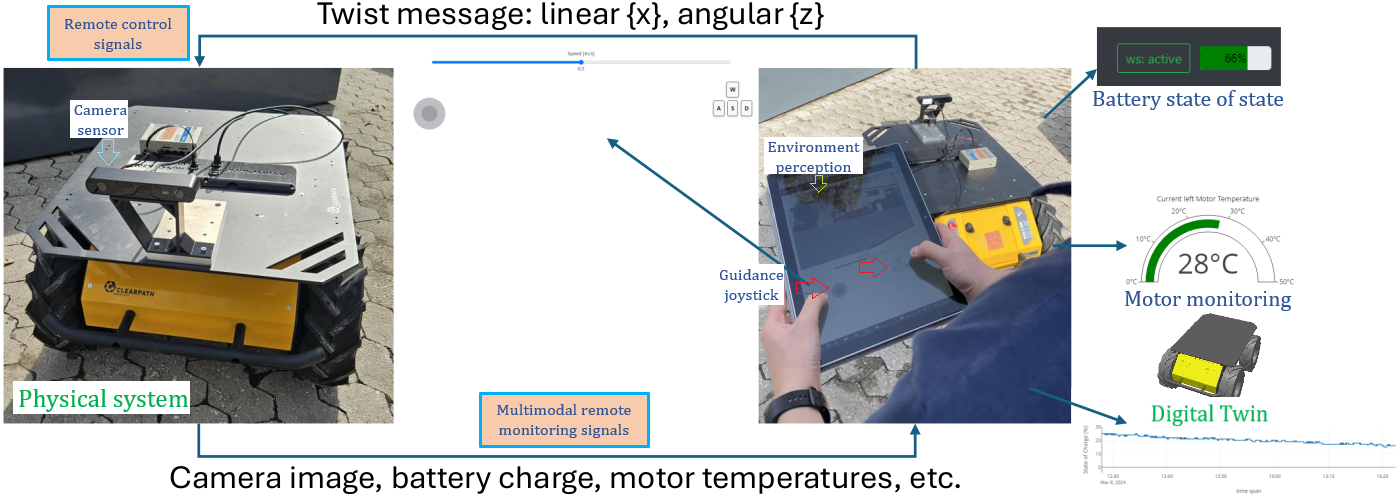
\includegraphics[width=18.2cm]{Pictures/loop.png}}
    \caption{Data loop between the Husky UGV robot and the web user interface}
    \label{fig:loop}
\end{figure*}

\begin{figure}[htbp]
    \centerline{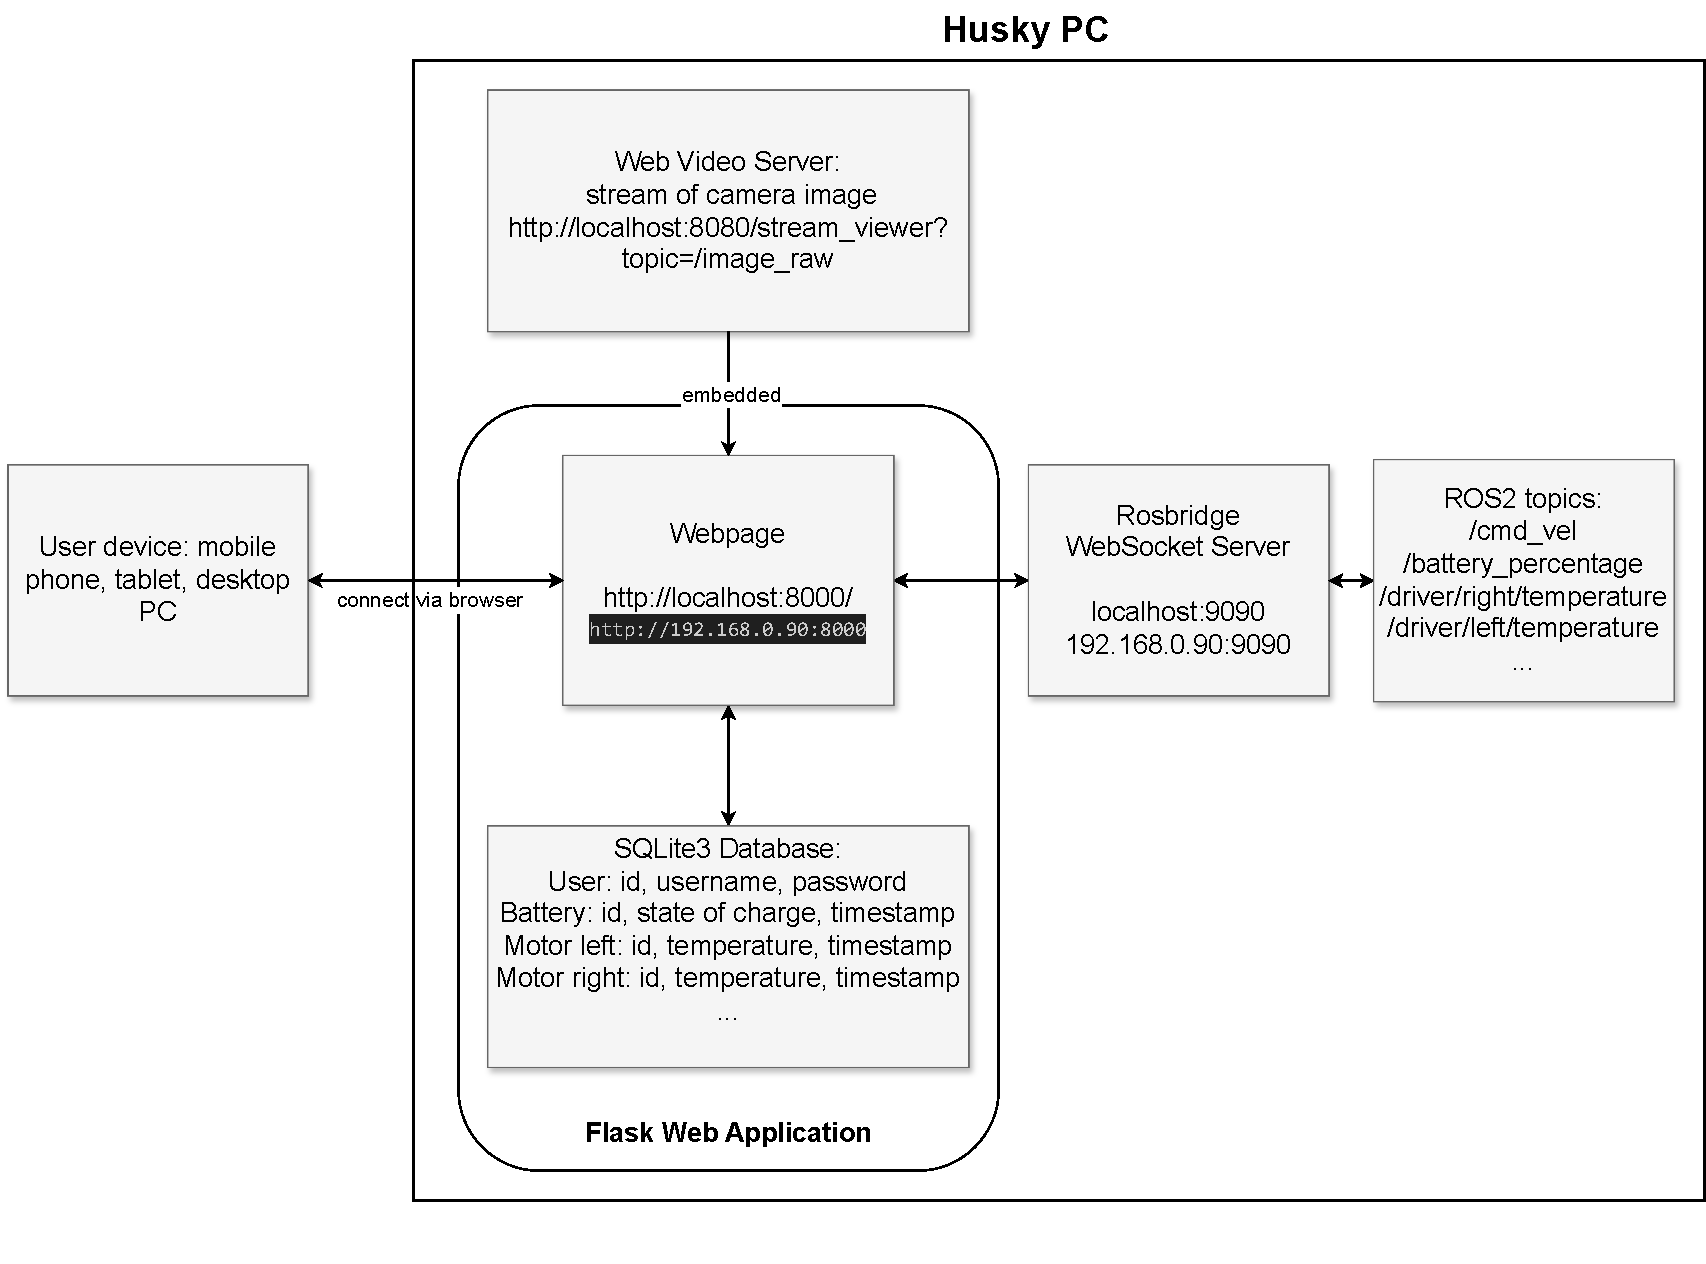
\includegraphics[width=8.9cm]{Pictures/userapp.pdf}}
    \caption{Backend architecture of the web app}
    \label{fig:userapp}
\end{figure}
Fig. \ref{fig:userapp} illustrates the backend architecture and the method by which users can interface with the Husky robot via the web application. This system is designed to operate on any device equipped with a web browser, utilizing the IP address of the Husky's onboard computer for connectivity.
The user interface provides real-time access to a stream of visual data from a Zed 2i camera as well as control options for the robot. Additionally, it displays current ROS data, including metrics such as the battery State of Charge (SoC) and motor temperatures.
A key feature of this system is its ability to track and store historical data in the SQLite database. This allows for longitudinal analysis of the robot's operational data, which can be instrumental in performance optimization and troubleshooting.
This system provides a flexible and accessible platform for robot control and data monitoring. It underscores the potential of web-based interfaces in enhancing the usability and functionality of robotic systems. 
The use of an IP-based connection protocol further emphasizes the system's adaptability and broad accessibility. The incorporation of a database for data tracking and storage demonstrates a commitment to data-driven decision making and performance optimization. 

\subsection{Frontend}
The primary objective of the frontend design is to enhance user-friendliness through visually intuitive components. Additionally, the application aims for platform independence, ensuring that users are not constrained by specific devices when accessing the web user interface. 
To achieve this, the web application is crafted to be compatible with a wide range of devices including desktop PCs and mobile devices. The result of the individual frontend design tools presented here are shown in \ref{VS}.
\begin{itemize}
\item Leveraging the free and open-source CSS framework Bootstrap version 4.6, we optimize responsiveness and seamlessly integrate with prevailing web standards such as HTML5, CSS3, and JavaScript \cite{bootstrap}. 
In the context of Bootstrap, the layout structure is organized using the grid system for arranging elements and components within a web page. 
Additionally, a navigation bar is crafted to reinforce user navigation.
Furthermore, the implementation of a battery display is achieved through the utilization of the Bootstrap class .progress-bar. 
This class enables precise control over visual representations of battery levels or other progress indicators.
\item Plotly.js, an open-source graphing library serves as a powerful tool for constructing interactive and touch-enabled visualizations. It facilitates the creation of dynamic plots that allow users to zoom in and out as well as capture screenshots of relevant data \cite{plotly}.
\item The Husky is supplied with a physical controller as standard. Teleoperation is achieved through the utilization of an analog joystick and the left and right shoulder buttons to set a specific maximum velocity \cite{huskydriving}.
To extend this functionality to the web interface, Nipple.js is employed. This library empowers the configuration and display of a virtual joystick \cite{nipplejs}. Additionally, a horizontally scrollable velocity slider is created using the Bootstrap class .form-control-range to set a desired maximum speed.
\item The app exhibits versatility in its control mechanisms. Users have the option to teleoperate the robot via a physical keyboard, provided they have one readily available. For users lacking a physical keyboard connection, an alternative method involves utilizing the custom “WASD” touch keys displayed within the application interface. 
These touch keys can also be used for the robot movement. The Husky can be driven more precisely using the keyboard buttons. This can be useful when parking, for instance.
\item Three.js is a powerful and lightweight 3D graphics library that can be served as a versatile tool for rendering digital representations of robots within web browsers \cite{threejs}. In future work a combination with Ros3djs can be considered to create a digital twin in the browser that mirrors the physical movements of the real robot \cite{ros3djs}. Animations can also be added. For example, a blinking or lighting up of the visualized husky in the browser when the battery SoC is low. 
As an ongoing project, we have successfully integrated a 3D model of the Husky into our application as a proof of concept (Fig. \ref{fig:3dreal}).
\end{itemize}

\subsection{Interaction between backend and frontend}
The value of the battery SoC is used as an example to explain the data flow between the backend and frontend. 
\subsubsection{Direct display of the battery SoC}
The current value of the battery SoC which is published by the ROS topic /battery\_percentage is visualized directly in the user interface with Bootstrap each time the message is received. For this purpose, a ROSLIB.topic object is created beforehand in JavaScript that subscribes to the corresponding ROS topic, allowing real-time updates. It is also possible to send messages to this topic, as is the case with the Husky teleoperation. 
In this case the virtual joystick position sends a twist message to the /cmd\_vel topic to move it. 
The connection between the app and the Husky is established via the WebSocket. 
\subsubsection{Capturing the values}
In the backend, a route is defined in the Flask web application that listens for HTTP POST requests at the /save\_data endpoint. If a POST request is received, the incoming JSON data is queried. In this scenario, a battery object is then created with the percentage value and adds it with an id and a timestamp to the database session (Fig. \ref{fig:userapp}). In the event of a database failure, the current battery SoC can still be displayed. The same applies to the engine temperatures (Fig. \ref{fig:backfront}).
\subsubsection{Visualizing the data from the database}
The SoC for the battery is visualized using Plotly.js as a line chart. This process involves several steps. Initially, data is fetched from the backend database. After processing to ensure compatibility with Plotly.js, it is prepared for visualization. The resulting line diagram represents the battery SoC over a certain time span. Flask facilitates the transfer of Python variables to the frontend. 
These variables are utilized within HTML templates or JavaScript via Jinja, a template engine. Users can interact with the system by selecting specific days from a drop-down list. The recorded data corresponding to the chosen day is displayed.
\begin{figure}[tp]
    \centerline{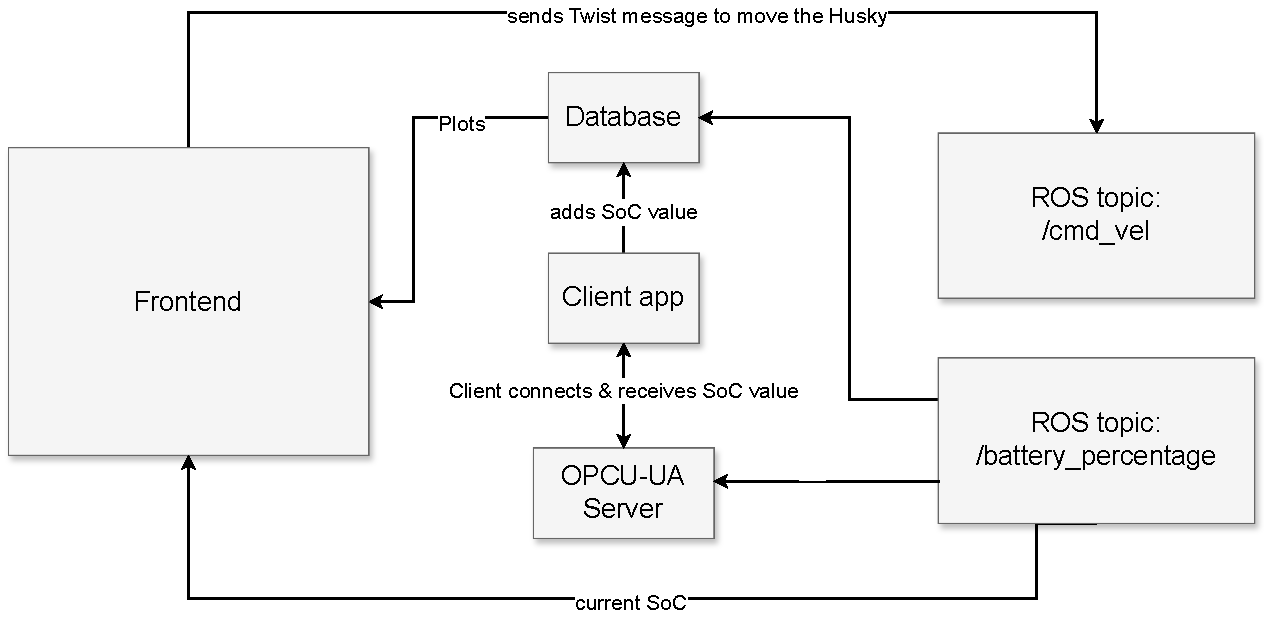
\includegraphics[width=8.9cm]{Pictures/backfront.pdf}}
    \caption{Interaction between frontend and backend}
    \label{fig:backfront}
\end{figure}
\subsubsection{Connecting to an Open Platform Communications Unified Architecture Server}
A pre-existing DataConnector (DC) has been specifically developed for the Husky as part of a prior project. This DC leverages the Open Platform Communication Unified Architecture (OPC-UA) standard. Through this connector, the ROS data from the Husky can be efficiently retrieved. The retrieval process is facilitated by a client program integrated into the web application and the acquired data is persistently stored in the database. 
In the event of an OPC-UA server failure, the system is designed to continue displaying the real-time ROS data of the Husky (Fig. \ref{fig:backfront}).


\section{Validation and Showcase}\label{VS}
To test the responsiveness of the front end of the web application, the app was accessed from different devices. The Flask application can run on the Husky's onboard PC or on another PC in the same local network as the Husky with access to the ROS topics. The application was mainly tested on the mobile onboard PC (i5-1135G7 CPU and 16 GB RAM) to serve the locally stored files to the client.
The representation of the data page is shown in Fig. \ref{fig:galaxysurface}. 
\begin{figure}[htbp]
    \centerline{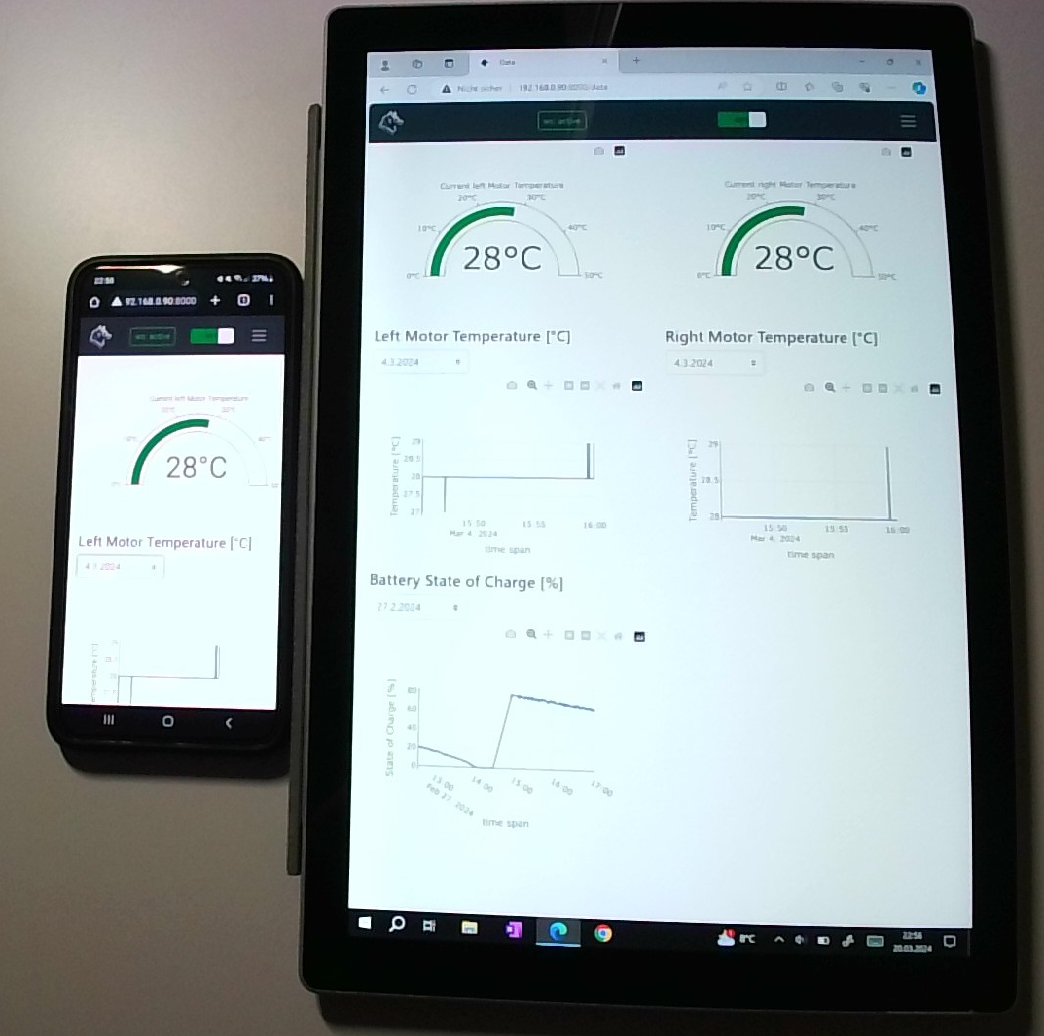
\includegraphics[width=8.8cm]{Pictures/galaxysurfacecut.png}}
    \caption{Galaxy S23 mobile view on the left and Surface Pro (5th Gen.) view on the right.}
    \label{fig:galaxysurface}
\end{figure}
In this experiment we investigate the visual representation of the web application interface across two distinct devices: a Samsung Galaxy S23 cell phone and a Microsoft Surface Pro tablet (5th Gen.). The purpose is to discern how design elements and user experience differ between these platforms.
On the left hand side the /data page was accessed using a Samsung Galaxy S23 cell phone while on the right hand side the site was displayed on the Surface Pro tablet.
Embedded within the navigation bar is a real-time indicator of the battery SoC at the top right corner. This value is updated dynamically as the Husky operates.
Additionally, a status display reflects the active WebSocket connection (next to the SoC), providing essential feedback to the user.
These components were crafted using the Bootstrap framework. The current motor temperatures are visualized using angular gauge charts. These succinct representations allow rapid assessment of temperature levels.
Below that, the motor temperature data are plotted as line charts. Both visualizations were generated using Plotlyjs.
Positioned at the bottom left corner, a similar display exists for the battery SoC which can be seen on the Surface Pro tablet. Due to space constraints of the Galaxy S23 screen only a truncated version of the data page is visible in Fig. \ref{fig:galaxysurface}. To view the remaining gauge and plots on the Galxy S23 view it is required to scroll down. The visualizations are listed below each other.  
On both devices, the navigation bar undergoes compression, resulting in a more compact layout.
A convenient drop-down menu arrangement (top right) allows users to access elements sequentially by scrolling vertically.\\
The control interface in Fig. \ref{fig:galaxycontrol} features a live image display of a Zed 2i camera, which serves as the primary view. Positioned centrally, this display provides real-time visual feedback. Beneath the image, the speed slider resides. The speed slider is adjustable from 0.1 meter per second to a maximum of 1 meter per second and is accompanied by a numerical readout.
The interface includes touch-enabled controls: a virtual joystick positioned at the bottom left and virtual keyboard keys at the bottom right. These intuitive input mechanisms facilitate precise guidance control of the Husky robot. 
Their placement at the screen's edge aligns with the ergonomic orientation of handheld devices such as cell phones or tablets, enhancing user comfort and efficiency. 
\begin{figure}[htbp]
    \centerline{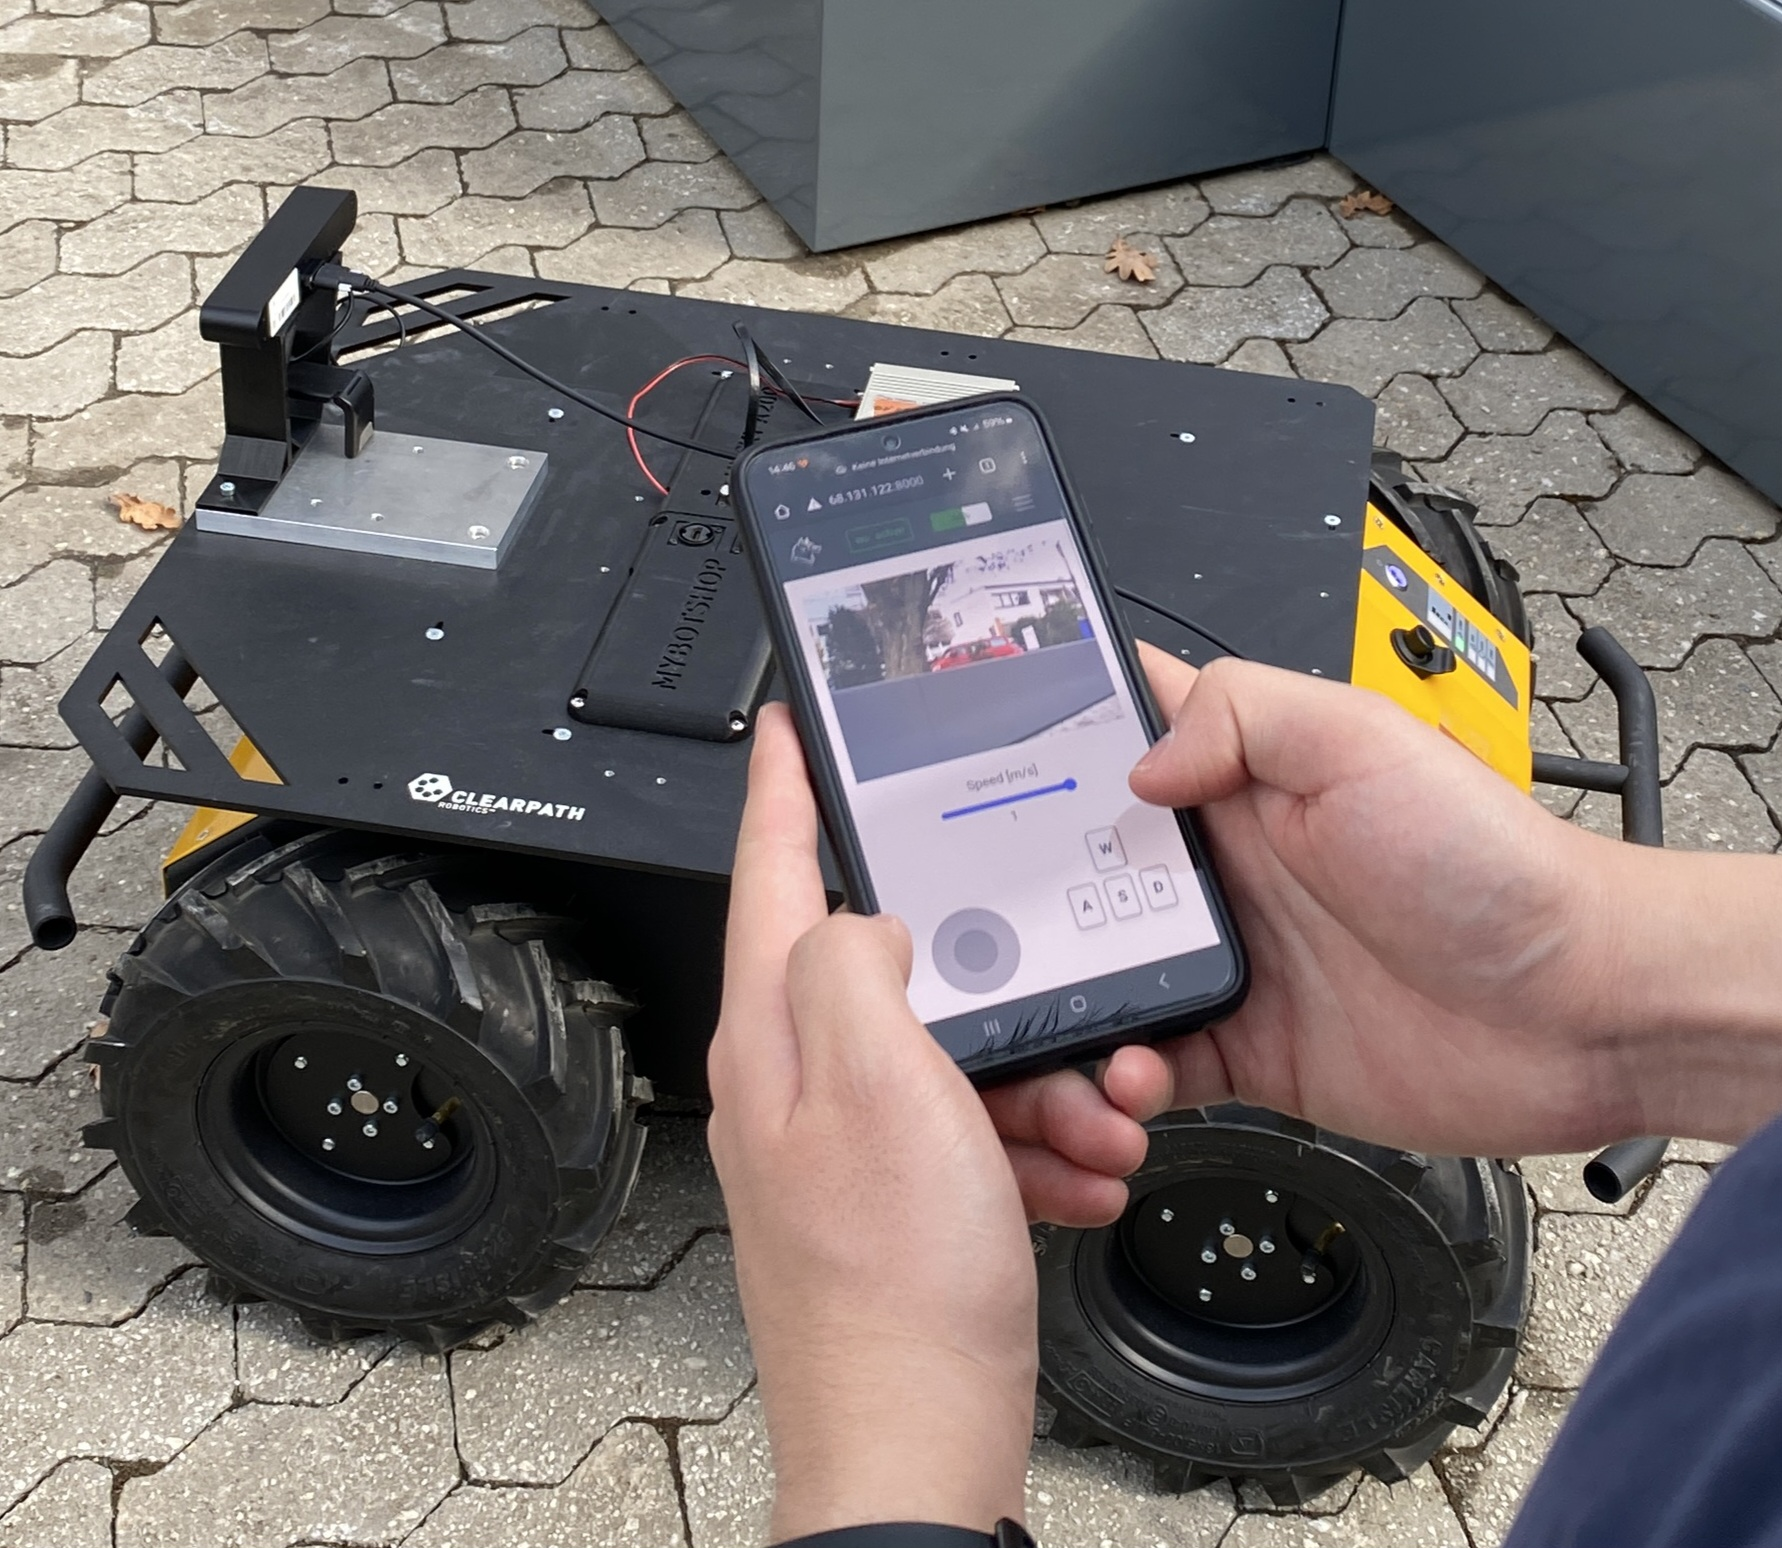
\includegraphics[width=8.9cm]{Pictures/galaxycontrol.jpg}}
    \caption{Control panel (mobile view with Galaxy S23) with battery soc, WebSocket status, live camera image, virtual Joystick, speed slider and virtual keyboard keys.}
    \label{fig:galaxycontrol}
\end{figure}
The 3D model route shows the visualized Husky as depicted in Fig. \ref{fig:3dreal}. It is possible to view the model from different angles.
The components listed here have been tested with the most common browsers such as Chrome, Firefox or Edge in different versions and on different devices. A list of supported browser versions of the Bootstrap components is available on the Bootstrap webpage \cite{bsBrowsers}. 
\begin{figure}[htbp]
    \centerline{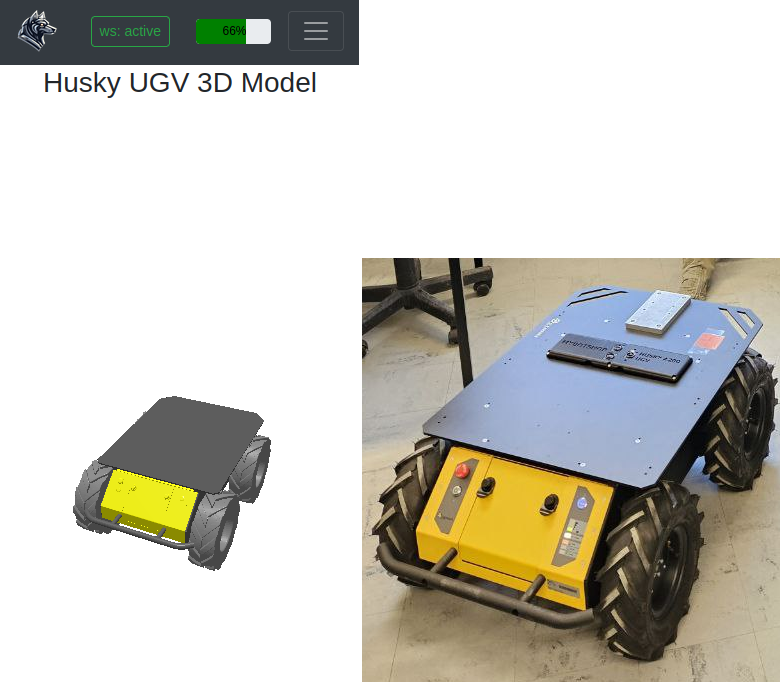
\includegraphics[width=8.9cm]{Pictures/3dreal.png}}
    \caption{Husky 3D model inside the application (mobile view) on the left and the physical Husky on the right}
    \label{fig:3dreal}
\end{figure}
\section{Conclusion}
This work has aimed to develop a web-based application that facilitates user interaction with the Husky robot. The primary objectives include providing an intuitive interface for comprehending the robot's internal mechanisms and environmental context, as well as enabling versatile control over its operations. 
Notably, compatibility considerations extend to diverse devices with web connectivity, irrespective of their origin or browser specifications. The application integrates a robust database, empowering users to monitor and derive informed decisions from real-time robot data. 
Additionally, visual representations enhance the presentation of critical parameters, such as motor temperature and battery status.
[Evtl. Outlook-Part hier]

\begin{thebibliography}{00}
\bibitem{rosOrg}"ROS - Robot Operating System," ROS, https://ros.org (accessed March 18, 2024).
\bibitem{huskyClearpath}"Husky UGV - Outdoor Field Research Robot by Clearpath," Clearpathrobotics, https://clearpathrobotics.com/husky-unmanned-ground-vehicle-robot/ (accessed March 17, 2024).
\bibitem{kapic} Zinaid Kapić, Aladin Crnkić, Edin Mujčić and Jasna Hamzabegović, "A web application for remote control of ROS robot based on WebSocket protocol and Django development environment", in IOP Conf. Ser.: Mater. Sci. Eng. 1208 012035, 2021, doi: 10.1088/1757-899X/1208/1/012035.
\bibitem{rosbridgeOkState} Crick, C., Jay, G., Osentoski, S., Pitzer, B., and Jenkins, O. C. "Rosbridge: Ros for non-ros users" in Robotics Research, Springer, 2017, pp. 493--504.
\bibitem{rosbridgeSuite}"rosbridge\_suite," ROS, http://wiki.ros.org/rosbridge\_suite (accessed March 14, 2024).
\bibitem{dinodi} D. D. Rajapaksha et al., "Web Based User-Friendly Graphical Interface to Control Robots with ROS Environment," 2021 6th International Conference on Information Technology Research (ICITR), Moratuwa, Sri Lanka, 2021, pp. 1-6, doi: 10.1109/ICITR54349.2021.9657337.
\bibitem{johnson}Brisaac Johnson et al., "Towards Web-based Environments for Prototyping Social Robot Applications," in Companion of the 2021 ACM/IEEE International Conference on Human-Robot Interaction (HRI '21 Companion). Association for Computing Machinery, New York, NY, USA, 308-312, https://doi.org/10.1145/3434074.3447182.
\bibitem{webvideoserver}"web\_video\_server," ROS, http://wiki.ros.org/web\_video\_server (accessed March 20).
\bibitem{wang}X. Wang et al., "TeleRobot: Design and Implementation of a Live Remote Interaction Platform for Robots*," 2023 IEEE International Conference on Systems, Man, and Cybernetics (SMC), Honolulu, Oahu, HI, USA, 2023, pp. 408-412, doi: 10.1109/SMC53992.2023.10394406.
\bibitem{flasksqlite} Suraya, Muhammad Sholeh, "Designing and Implementing a Database for Thesis Data," in International Journal of Engineering, Science \& InformationTechnology (IJESTY) Volume 2, No. 1, 2022, pp. 9--14, eISSN: 2775-2674.
\bibitem{sqlalchemy}"The Python SQL Toolkit and Object Relational Mapper," SQLAlchemy, https://www.sqlalchemy.org/ (accessed March 20, 2024).
\bibitem{sqlite}"About SQLite," SQLite, https://www.sqlite.org/about.html (accessed March 20, 2024).
\bibitem{twistmsg}"geometry\_msgs/Twist Message," ROS docs, https://docs.ros.org/en/diamondback/api/geometry\_msgs/html/msg/\\Twist.html (accessed March 19, 2024).
\bibitem{huskydriving}"Driving a Robot," Clearpath Robotics docs, https://docs.clearpathrobotics.com/docs/ros/tutorials/driving (accessed March 19, 2024).
\bibitem{flasklogin}"Flask-Login," flask-login readthedocs, https://flask-login.readthedocs.io/en/latest/ (accessed March 20, 2024).
\bibitem{werkzeug}"Utilities," Werkzeug, https://werkzeug.palletsprojects.com/en/\\2.3.x/utils/\#module-werkzeug.security (accessed March 20, 2024).
\bibitem{bootstrap}"Introduction," Bootstrap, https://getbootstrap.co, m/docs/4.6/getting-started/introduction/ (accessed March 16, 2024).
\bibitem{plotly}"Plotly JavaScript Open Source Graphing Library," Plotly, https://plotly.com/javascript/ (accessed March 21, 2024).
\bibitem{nipplejs}"nippleJS," NippleJS by yoannmoi, https://yoannmoi.net/nipplejs/ (accessed March 21, 2024).
\bibitem{threejs}"Creating a scene," threejs docs, https://threejs.org/docs/index.html\\\#manual/en/introduction/Creating-a-scene (accessed March 21, 2024).
\bibitem{ros3djs}"3D Visualization Library for use with the ROS JavaScript Libraries," ros3djs - ROS Wiki, http://wiki.ros.org/ros3djs (accesssed March 21, 2024).
\bibitem{bsBrowsers}"Browsers and devices," Getbootstrap, https://getbootstrap.com/docs/4.6/getting-started/browsers-devices/ (accessed March 17, 2024).
\end{thebibliography}
\vspace{12pt}


\end{document}
